% Definición
\documentclass[10pt]{beamer}

%For add subfigures
\usepackage{subcaption}

% Notas
\usepackage{pgfpages}
\setbeameroption{show notes on second screen=right}

% Datos
\title{Clasificador Documentos Médicos HOPE}
\subtitle{Trabajo Final De Máster, Área 2}
\author{Rubén Vasallo González}
\institute{UOC}
\date{\today}

% Temas
\usetheme{metropolis} % tema de presentación
\usecolortheme{default} % tema de color
\usefonttheme{default} % tema de fuente
\useinnertheme{default} % tema interior
\useoutertheme{default} % tema exterior


% Opciones
\setbeamertemplate{navigation symbols}{}
%\setbeamertemplate{background}{
\includegraphics[width=\paperwidth,height=\paperheight,keepaspectratio]{images/background.jpg}}

% Inicio
\begin{document}

{
\usebackgroundtemplate{
\includegraphics[width=\paperwidth]{images/background.jpg}}
\begin{frame}{Titulo}
  \maketitle
\end{frame}
} 

% Diapositivas
\begin{frame}{Índice}
  \setbeamertemplate{section in toc}[sections numbered]
  \tableofcontents[hideallsubsections]
  \note{
  Presentar proyecto ayuda a profesionales sanitarios encontrar referencias bibliográficas. \newline 
  \textbf{Intro}: Explicaremos los objetivos. \newline 
  \textbf{Metodología}: Analizaremos los datos y comentaremos problemas que nos han surgido durante el proyecto y como los hemos solventado. \newline 
  \textbf{Modelos Predictivos}: Veremos 3 modelos predictivos analizados. \newline 
  \textbf{Conclusiones}: Comentaremos las conclusiones finales.
  }
\end{frame}
 
\section{Introducción}

\begin{frame}{Introducción}
  \begin{itemize}
    \item Ayudar a los profesionales sanitarios a encontrar referencias bibliográficas adaptadas y personalizadas al paciente.
    \item Ayudar al proyecto HOPE a mejorar su algoritmo de Inteligencia Artificial (NLP).
  \end{itemize}
  \note{
  El master nace con el objetivo de poder ayudar a HOPE a recomendar referencias bibliográficas en base al feedback obtenido de los propios profesionales sanitarios. \newline
  HOPE: (Health Operations for Personalized Evidence) basado en (NLP) identifica la información clave de casos clínicos y referencias bibliográficas registradas en la Historia Clínica Electrónica. Pero no siempre acaba obteniendo referencias utiles para los casos personalizados. \newline
  Actualmente profesionales sanitarios dan feedback de esas recomendaciones y se quiere aprovechar esa información para mejorar el algoritmo.
  }
\end{frame}

\begin{frame}{Objetivos}
  \begin{itemize}
    \item<1-> \textbf{(OP)} Recomendar al profesional sanitario las referencias bibliográficas actuales útiles y personalizadas pudiendo realizar una clasificación (ranking) de más interés a menos.
    \item<2> \textit{(OS)} Analizamos el Conjunto de datos y componentes.
    \item<2> \textit{(OS)} Enriquecemos el conjunto de datos.
    \item<2> \textit{(OS)} Analizamos 3 posibles modelos predictivos.
    \item<2> \textit{(OS)} Realizamos la recomendación final
  \end{itemize}
  \note<1>{
  El objetivo es poder recomendar al profesional sanitario referencias bibliográficas ordenadas de más interés (utilidad) a menos. \newline
  Objetivo principal, entrenar un modelo predictivo basado en series temporales para poder realizar la clasificación por ranking.
  }
  \note<2>{
  Para ello analizaremos el conjunto de datos y sus componentes (atributos). \newline
  Intentamos enriquecer el conjunto debido a su poco volumen de datos. \newline
  Analizamos ...
  }
\end{frame}
 
\section{Metodología}
 
\begin{frame}{Conjunto de Datos}
  \begin{itemize}
    \item \textbf{age}: 75,86,40,...
    \item \textbf{diagnostic\_main}: Fistula Peritoneal, Insuficiencia Respiratoria,...
    \item \textbf{gender}: male
    \item \textbf{artículo}: 28694230,28805236,...
    \item \textbf{articlesRevisedYear}: 2018,2017,2016,...
    \item \textbf{articlesRevisedMonth}: 4,12,6,9,...
    \item \textbf{pubmed\_keys}: (Abdomen, Adenocarcinoma, Antiemetics, Blood), (Abdomen, Analgesics, Bone, Catharsis), (Abdomen, Anti-Bacterial Agents, Diuresis),...
    \item \textcolor{red}{\textbf{utilidad}}: 0,1,NA
  \end{itemize}
  \note{
  - Conjunto de datos con muchísimos atributos en formato documento y sin que persistan en todas las observaciones. \newline
  - Se decide junto al cliente escoger los atributos que mas se repiten en todas las observaciones, que son los que se muestran a continuación. \newline
  }
\end{frame}
 
\begin{frame}{Limitaciones encontradas}
  \begin{itemize}
    \item Poco volumen de información (51 obs. con atrb. \textit{utilidad} informado).
    \item Atributo a predecir sin la información suficiente para poder hacer un \textit{ranking}.
    \item Conjunto de datos Sesgado.
  \end{itemize}
  \begin{figure}[!htb]
    \begin{subfigure}[b]{0.45\linewidth}
    	\centering
	    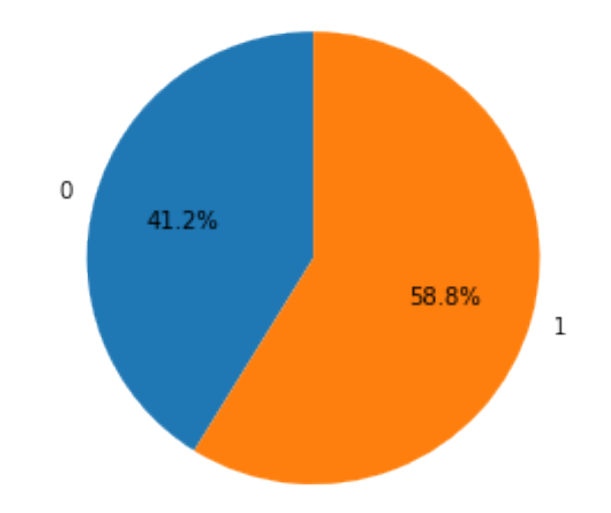
\includegraphics[width=0.9\textwidth]{images/sesgado_1.png}
	    \caption{Atributo \textit{utilidad}}
	\end{subfigure}
	\begin{subfigure}[b]{0.45\linewidth} 
		\centering
		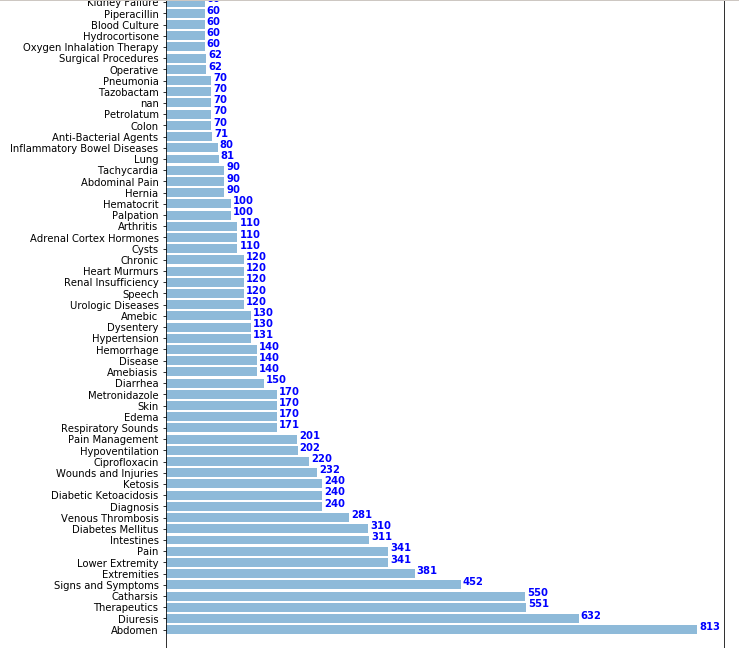
\includegraphics[width=0.9\textwidth]{images/sesgado_2.png}
			    \caption{Atributo \textit{pubmed\_keys}}
	\end{subfigure}
  \end{figure}
  \note<1>{
  - Conjunto de datos con poco volumen. \newline
  - No todas las observaciones tienen indicado el atributo a predecir (utilidad). \newline
  - No se puede realizar un \textit{ranking} con la información actual. \newline
  - Para intentar ganar algo de volumen se decide expandir el atributo pubmed\_keys para
  - Se decide con el cliente hacer un clasificador binario para indicar si el articulo es útil o no. Si se consigue el detalle de la utilidad durante el transcurso del ejercicio se volvería a objetivo principal. \newline
  - Como existen observaciones sin el atributo utilidad, se acuerda intentar enriquecer el conjunto de datos basándonos en los atributos que si tienen informado el atributo a predecir. \newline
  - También se decide generar un segundo conjunto de datos partiendo del conjunto de datos original pero expandiendo el atributo \textit{pubmed\_keys} para ver si la información de ese atributo a nivel individual puede ser un valor determinante.
  
  }
  \note<2>{
  - Se observa el conjunto de datos sesgado en el atributo a predecir y en el atributo \textit{pubmed\_keys}. Esto afectara a que la mayoría de modelos seguramente estarán sobreajustados.
  }
\end{frame}

\begin{frame}{Análisis de componentes principales (PCA)}
  \begin{itemize}
  	\item \textbf{Conjunto 1}: Dataset Completo
  	\item \textbf{Conjunto 2}: Dataset Completo pero añadiendo el mes y año del artículo y cogiendo solo las observaciones que se ha informado el atributo utilidad.
  	\item \textbf{Conjunto 3}: Dataset conjunto 2 pero eliminando los atributos \textit{gender} y artículo y se expande el atributo \textit{pubmed\_keys}
  \end{itemize}
  \note{
  - Conjunto 1 con age, diagnostic\_main, gender, artículo, pubmed\_keys y utilidad. \newline
  - Conjunto 2 añadiendo el mes y año del artículo y cogiendo solo las observaciones que se ha informado el atributo utilidad. \newline
  - Conjunto 3 
  }
\end{frame}

\begin{frame}{Análisis de componentes principales (PCA)}
  \begin{itemize}
  	\item Se Transformo todos los atributos Categóricos (texto) a Continuos (números continuos).
  	\item Se estandarizó los valores a un rango de entre 1 y -1.
  	\item Para el entrenamiento de los modelos predictivos, se dividió el conjunto en dos grupos. 1 Grupo de entrenamiento con el 75\% de observaciones. 2 Grupo para la validación con el 25\% de observaciones.
  \end{itemize}
  \note{}
\end{frame}

\begin{frame}{Resultados del análisis de componentes principales (PCA)}
  \begin{itemize}
  	\item Conjunto 1: Con solo \textbf{3 atributos}, el modelo es capaz de \textbf{explicar (predecir) el 95\%} de las observaciones.
    \begin{figure}[!htb]
      \centering
      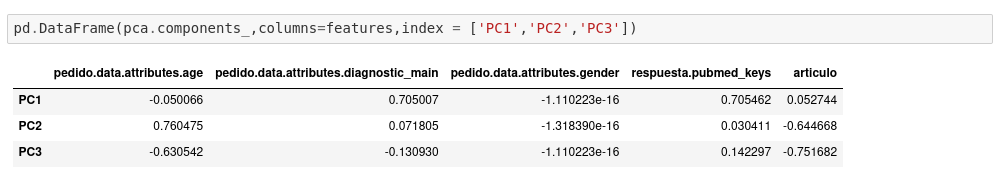
\includegraphics[width=0.9\textwidth]{images/resultados_procesado_de_datos_pca1_atributos.png}
    \end{figure}
    \item Conjunto 2: Con \textbf{5 atributos}, el modelo es capaz de \textbf{explicar (predecir) el 97\%} de las observaciones.
    \begin{figure}[!htb]
      \centering
      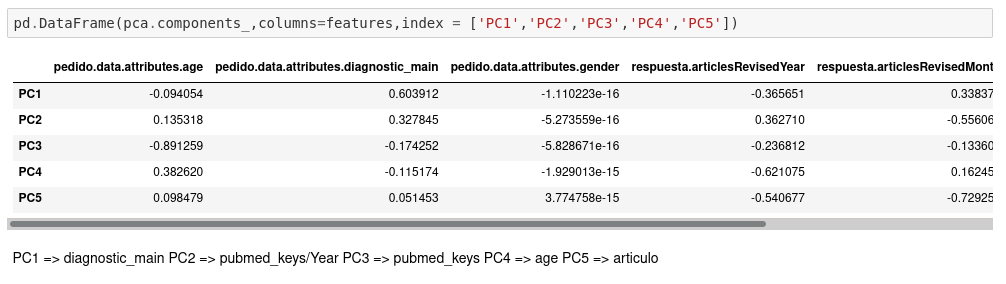
\includegraphics[width=0.9\textwidth]{images/resultados_procesado_de_datos_pca2_atributos.png}
    \end{figure}
  \end{itemize}	
  \note{
  La diferencia entre el conjunto 1 y 2 seguramente este debido a que el conjunto completo contiene un gran volumen de observaciones con el atributo \textit{utilidad} sin definir, lo que hace que prácticamente cualquier
valor que tengan los atributos se acaben asociando a un resultado sin definir.
  }
\end{frame}

\begin{frame}{Resultados del análisis de componentes principales (PCA)}
  \begin{itemize}
  	\item Conjunto 3: Con solo \textbf{4 atributos}, el modelo es capaz de \textbf{explicar (predecir) el 90\%} de las observaciones.
    \begin{figure}[!htb]
      \centering
      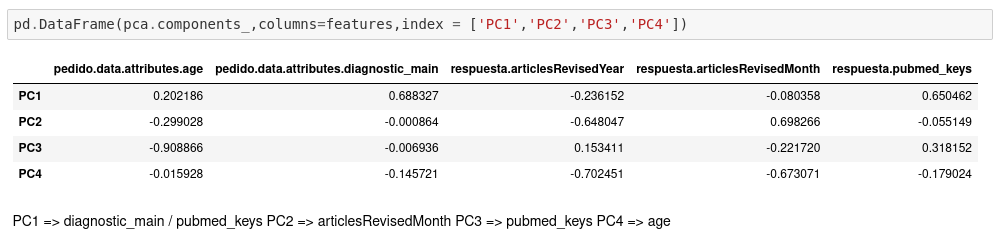
\includegraphics[width=0.9\textwidth]{images/resultados_procesado_de_datos_pca3_atributos.png}
    \end{figure}
  \end{itemize}	
  \note{Descartamos usar el conjunto 1 para los modelos debido a su gran volumen de resultados sin definir. Utilizaremos los otros dos conjuntos para analizar los resultados de los posteriores modelos.}
\end{frame}

\begin{frame}{Intentando enriquecer los datos (K-Nearest-Neighbor)}
  \begin{itemize}
  	\item \textbf{Conjunto 1}: Dataset Completo cogiendo solo las observaciones que se ha informado el atributo utilidad.
  	\item \textbf{Conjunto 2}: Dataset conjunto 1 pero eliminando los atributos \textit{gender} y artículo y se expande el atributo \textit{pubmed\_keys}
  \end{itemize}
  \note{
  - Conjunto 1 con age, diagnostic\_main, gender, artículo, mes y año del articulo, pubmed\_keys y cogiendo solo las observaciones que se ha informado el atributo utilidad. \newline
  - Conjunto 2
  - Se aplican a los dos conjuntos las transformaciones mencionadas anteriormente.
  }
\end{frame}

\begin{frame}{Resultados del enriquecimiento (K-Nearest-Neighbor)}
  \begin{itemize}
  	\item \textbf{Conjunto 1}: \textbf{K = 6} utilizando el calculo de la distancia '\textbf{distance}', con un porcentaje de acierto del \textbf{85\%}.
  	\item \textbf{Conjunto 2}: \textbf{K = 1} utilizando el calculo de la distancia '\textbf{uniform}', con un porcentaje de acierto del \textbf{90\%}.
  \end{itemize}
  \begin{figure}[!htb]
    \begin{subfigure}[b]{0.45\linewidth}
    	\centering
	    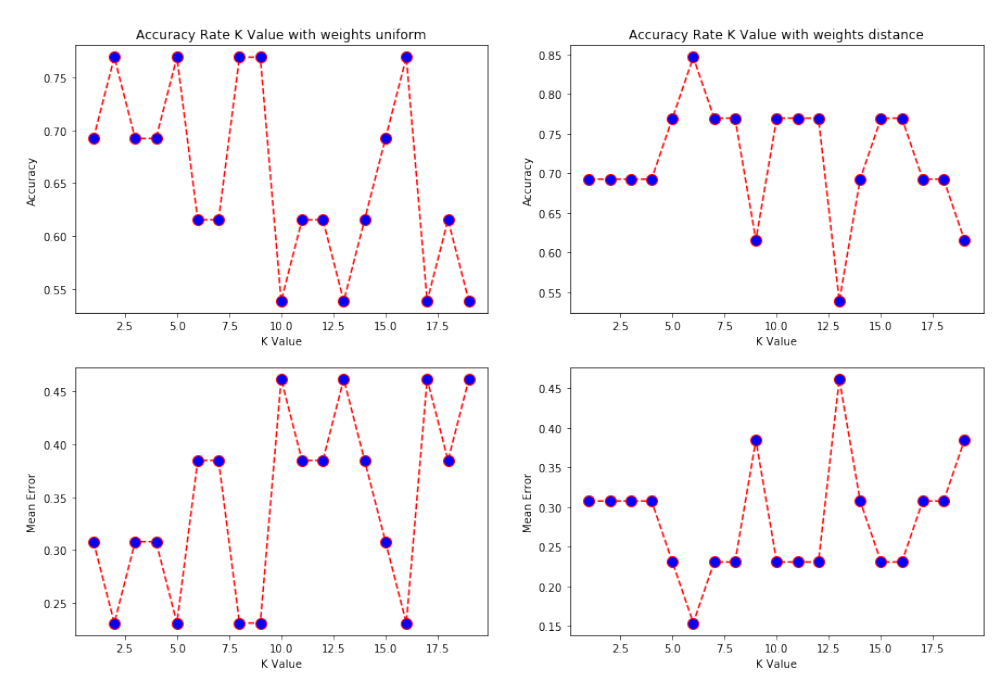
\includegraphics[width=0.9\textwidth]{images/resultados_knn_ent_conjunto1.png}
	    \caption{Conjunto 1}
	\end{subfigure}
	\begin{subfigure}[b]{0.45\linewidth} 
		\centering
		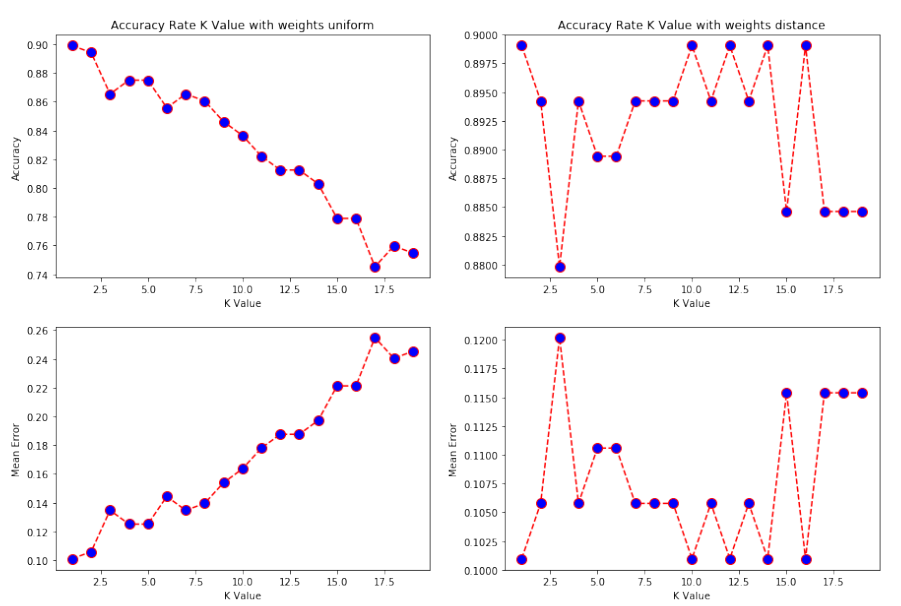
\includegraphics[width=0.9\textwidth]{images/resultados_knn_ent_conjunto2.png}
	    \caption{Conjunto 2}
	\end{subfigure}
  \end{figure}
 \note{
 - distance: Cuanto mas cerca, más probabilidad de pertenecer al grupo (mas peso). \newline
 - uniform: Todos los puntos tienen el mismo peso. \newline
 \newline
 Aconsejamos no utilizar el modelo, ya que los conjuntos se observan \textbf{sesgados} y esto puede afectar al entrenamiento de los posteriores modelos.
 }
\end{frame}

\section{Análisis Modelos Predictivos}

\begin{frame}{Conjuntos de datos para el estudio de los modelos}
  \begin{itemize}
  	\item \textbf{Conjunto 1}: Dataset Completo cogiendo solo las observaciones que se ha informado el atributo utilidad.
  	\item \textbf{Conjunto 2}: Dataset conjunto 1 pero eliminando los atributos \textit{gender} y artículo y se expande el atributo \textit{pubmed\_keys}
  \end{itemize}
  \textbf{Nota}: Se utilizaron los mismos conjuntos para los 3 modelos y se aplican las mismas transformaciones mencionadas anteriormente.
  \note{
  - Conjunto 1 con age, diagnostic\_main, gender, artículo, mes y año del articulo, pubmed\_keys y cogiendo solo las observaciones que se ha informado el atributo utilidad. \newline
  - Conjunto 2
  - Se aplican a los dos conjuntos las transformaciones mencionadas anteriormente.
  }
\end{frame}

\begin{frame}{Resultados del Modelo 1 (Regresión logística)}
  \begin{itemize}
  	\item \textbf{Conjunto 1}: Precisión del \textbf{65\%} sobre el conjunto de validación.
  	\item \textbf{Conjunto 2}: Precisión del \textbf{49\%} sobre el conjunto de validación.
  \end{itemize}
  \begin{figure}[!htb]
    \begin{subfigure}[b]{0.45\linewidth}
    	\centering
	    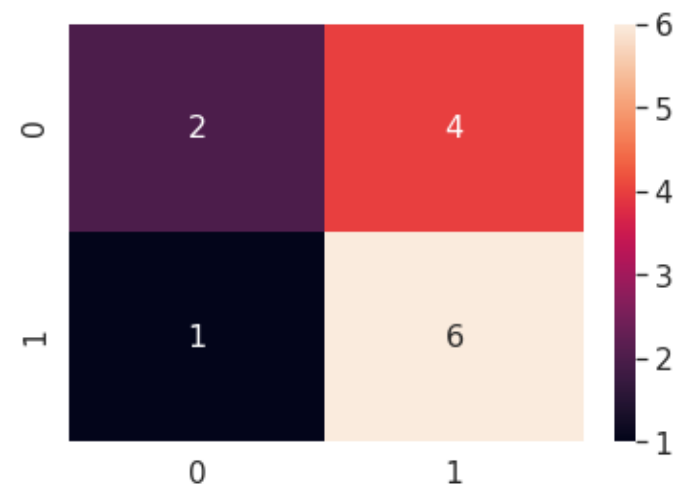
\includegraphics[width=0.9\textwidth]{images/resultados_lr_cm_conjunto1.png}
	    \caption{Conjunto 1}
	\end{subfigure}
	\begin{subfigure}[b]{0.45\linewidth} 
		\centering
		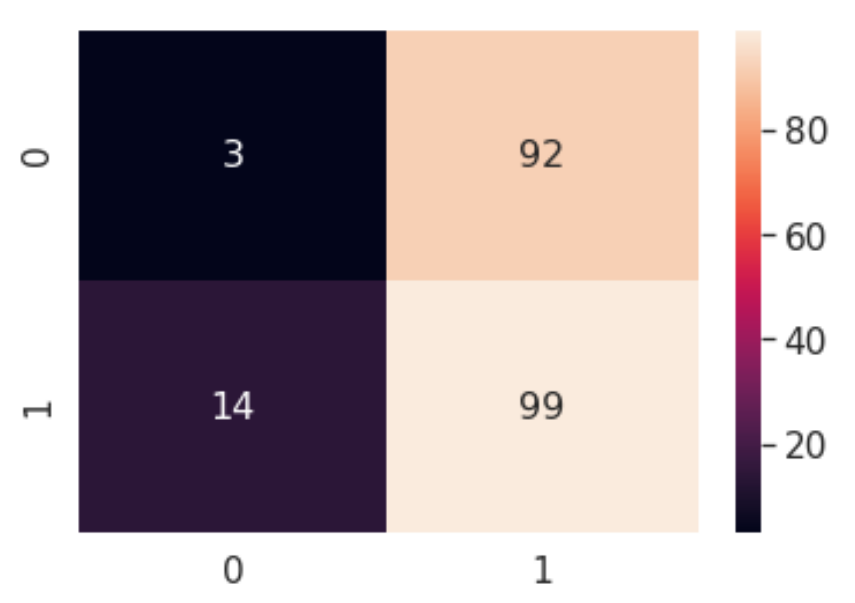
\includegraphics[width=0.9\textwidth]{images/resultados_lr_cm_conjunto2.png}
	    \caption{Conjunto 2}
	\end{subfigure}
  \end{figure}
  \note{Explicar Resultados Regresión logística}
\end{frame}

\begin{frame}{Resultados del Modelo 2 (Random Forests)}
  \begin{itemize}
  	\item \textbf{Conjunto 1}: \textbf{N\_Estimator: 40} con un porcentaje de acierto del \textbf{61\%}.
  	\item \textbf{Conjunto 2}: \textbf{N\_Estimator: 10} con un porcentaje de acierto del \textbf{89\%}.
  \end{itemize}
  \begin{figure}[!htb]
    \begin{subfigure}[b]{0.45\linewidth}
    	\centering
	    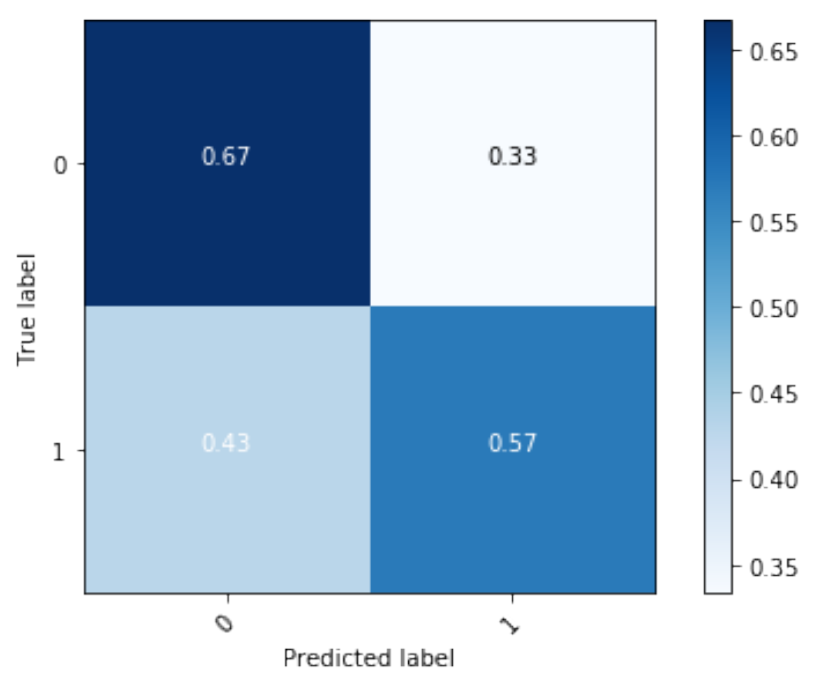
\includegraphics[width=0.9\textwidth]{images/resultados_rf_cm_conjunto1.png}
	    \caption{Conjunto 1}
	\end{subfigure}
	\begin{subfigure}[b]{0.45\linewidth} 
		\centering
		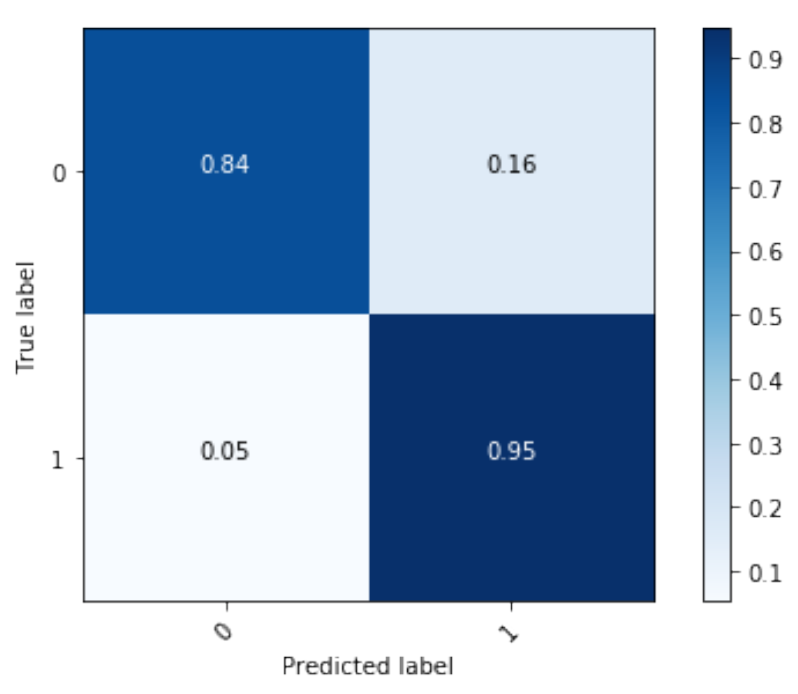
\includegraphics[width=0.9\textwidth]{images/resultados_rf_cm_conjunto2.png}
	    \caption{Conjunto 2}
	\end{subfigure}
  \end{figure}
  \note{
  - Se realiza el estudio del número de arboles que ha de tener el modelo para que este de su porcentaje de acierto mas elevado. \newline
  - Con el conjunto 2, el modelo se ajusta a unos resultados aceptables ya que esta lo suficientemente ajustado para que de resultados razonables sin estar sobreajustado.
  }
\end{frame}

\begin{frame}{Resultados del Modelo 3 (Support Vector Machines)}
  \begin{itemize}
  	\item \textbf{Conjunto 1}: \textbf{kernel: radial (rbf)} con un porcentaje de acierto del \textbf{54\%}.
  	\item \textbf{Conjunto 2}: \textbf{kernel: radial (rbf)} con un porcentaje de acierto del \textbf{89\%}.
  \end{itemize}
  \begin{figure}[!htb]
    \begin{subfigure}[b]{0.45\linewidth}
    	\centering
	    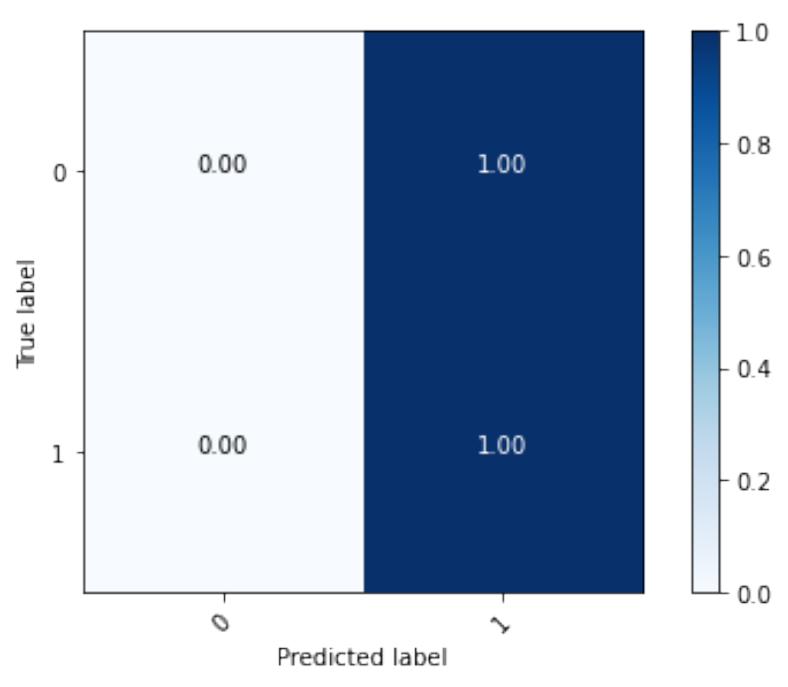
\includegraphics[width=0.9\textwidth]{images/resultados_svm_cm_conjunto1.png}
	    \caption{Conjunto 1}
	\end{subfigure}
	\begin{subfigure}[b]{0.45\linewidth} 
		\centering
		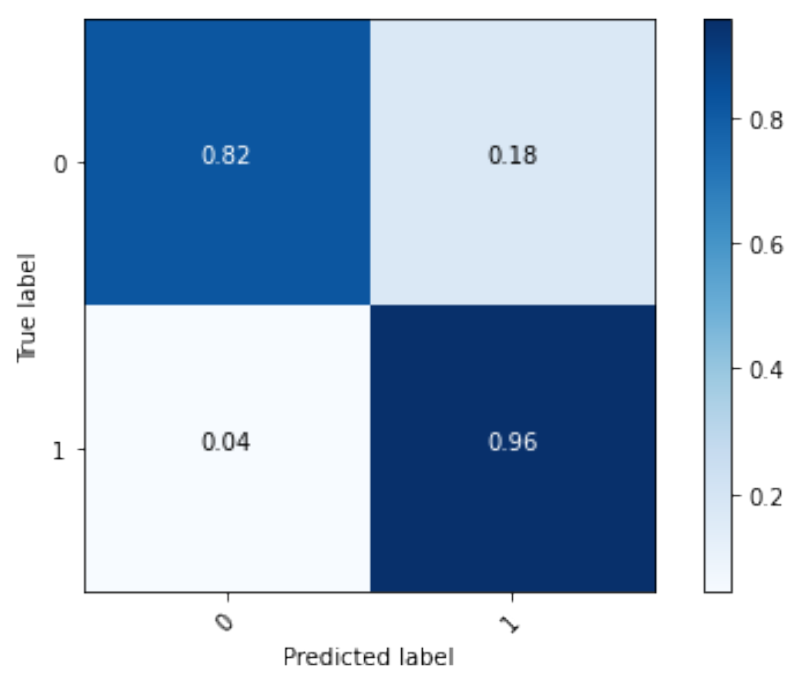
\includegraphics[width=0.9\textwidth]{images/resultados_svm_cm_conjunto2.png}
	    \caption{Conjunto 2}
	\end{subfigure}
  \end{figure}
  \note{
  - Se realizo un estudio de con los kernel 'polynomial', 'radial (rbf )' y 'sigmoid' y calculamos cuales son los mejores hiperparametros para cada uno de estos. \newline
  - Se observo que el kernel que mejor resultado era el radial y para el conjunto 2, el modelo se ajusta a unos resultados aceptables igual que ocurre para el caso del modelo de Random Forests.
  }
\end{frame}

\section{Conclusiones y Trabajos futuros}

\begin{frame}{Comparando los Modelos}
  \begin{table}[!htb]
	\begin{tabular}{ | p{2cm} | c | c | c | }
		\hline Modelos & Logit & \textbf{Bosques Aleatorios} & SVM \\ 
		\hline
		\hline
		Conjunto 1 & 65.78\% & 61.53\% & 53.85\% \\
		\textbf{Conjunto 2} & 49.03\% & \textbf{89.9\%} & 89.42\% \\ \hline
	\end{tabular}
  \end{table}
  \note{
  - El modelo que mejor precisión da es el Bosques aleatorios. \newline
  - Para poder predecir nuevos resultados, sera necesario aplicar a estos, las transformaciones que se han aplicado al conjunto 2.\newline
  Nota: No añadimos a la comparativa el modelo K-NN ya que, aunque se podría utilizar como modelo predictivo igual que en los otros casos, debido a que no se entreno con los mismos atributos que los otros modelos.
  }
\end{frame}

\begin{frame}{Trabajos futuro}
  \begin{itemize}
  	\item Mejorar el modelo actual.
  	\begin{itemize}
  	  \item Mejorar el actual modelo de Bosques aleatorios añadiendo más observaciones.
  	  \item Valorar si otros modelos predictivos tienen mejor resultado.
  	  \item Valorar si se altera la importancia de los atributos relevantes.
  	\end{itemize}
  	\item Entrenar un modelo capaz de realizar un ranking de utilidad.
  \end{itemize}
  \note{
  - Si se consiguen mas observaciones, se puede reentrenar el modelo de Bosques aleatorios para mejorar la predicción de este. \newline
  - Al conseguir mas observaciones, se puede probar con mas modelos para ver si alguno mejora la predicción del de Bosques aleatorios. \newline
  - Al añadir mas observaciones, puede ser que se altere la importancia de los atributos relevantes, por lo que conviene realizar el PCA cada cierto tiempo para comprobar si esto sucede.
  }
\end{frame}

{
\usebackgroundtemplate{
\includegraphics[width=\paperwidth]{images/background.jpg}}
\begin{frame}{Trabajos futuro}
  \huge
  Gracias por esta oportunidad
  
  \normalsize
  ¿Preguntas, dudas?
  
  \href{mailto:rvasallo@uoc.edu}{rvasallo@uoc.edu}
  
\end{frame}
}


\end{document}
